\section{Evaluation}\label{sec:results}

\rev{We evaluate RAMSES against existing serving stacks. Every experiment runs five times on the same hardware; tables report absolute request-level percentiles and run-level means with 95\% confidence intervals. All request-level latency, whole-node energy, operating-model, controller-ablation, and per-model results are computed by the released scripts from \texttt{artifact/data/actual/raw.jsonl}---16{,}000 records over eight configurations, five models, four task types, and five restarts---and the load-time/VRAM (Table~\ref{tab:loadtime_vram}), sensitivity, industrial-accuracy, and 72-hour QoS (Table~\ref{tab:qos}) series are released as measured CSVs, so every summary traces back to primary data rather than normalized plots.}

\subsection{Research Questions and Claim--Evidence Alignment}
\rev{We organize the evaluation around four questions tied directly to the
contributions in Section~\ref{sec:introduction}:}
\begin{description}
\item[RQ1: Predictive validity.] Do measured pressure ratios distinguish the regimes, and how accurately does the model predict held-out latency (coverage, MAE/RMSE)?
\item[RQ2: Value of switching.] Does state switching add value beyond the same mechanisms at fixed settings? The same-trace policy-off run is the counterfactual.
\item[RQ3: Benefit boundary.] Where does RAMSES improve latency, memory, failures, and energy, and where does its overhead cease to pay? We retain non-gains.
\item[RQ4: Semantic preservation.] Does relocation preserve outputs and named-task accuracy, paired on identical inputs?
\end{description}

\rev{Values under \texttt{artifact/data/expected/} are pre-experiment hypotheses used only to size the matrix; they are excluded from every table, figure, test, and claim, and unsupported configurations remain explicitly missing.}

\noindent\textbf{Testbed.}
Unless stated otherwise, the platform is a laboratory server, not a deployed factory-edge system:
two NVIDIA A100 (80GB) GPUs, an Intel Xeon Gold 6440 CPU (40 cores),
512~GB ECC DRAM, and a Gen4 NVMe SSD running PyTorch~2.4, CUDA~12.2,
and vLLM~0.5.3. Because vLLM~0.5.3 predates native Llama-4 support, we applied a compatibility patch that registers the Llama-4 model class and adapts the configuration and weight loaders; the patch and the exact invocation are included in the review artifact so the comparisons are reproducible. The principal workload is Llama-4 (Maverick-17B-128E-Instruct)~\cite{meta2025llama4}. Single-GPU ablations are flagged as ``1$\times$A100''.

Table~\ref{tab:baseline_comparison} captures the comparison scope.

% =====================================================


\subsection{Request-Level Measurement Methodology}
\label{sec:latency_protocol}
\rev{To prevent incompatible latency scales from being pooled, each request-level
record is assigned to exactly one task: \emph{scoring} (one forward pass, no
generation), \emph{continuation} (one warm decode step), \emph{TTFT} (request
arrival through first emitted token), or \emph{generation} (arrival through the
final token).  For every task and system we log the model, numerical precision,
input/output token counts, batch size, concurrency, request count, and run
identifier, following the schema in \texttt{../artifact/measurement-schema.json}.
From these logs the released analyzer computes absolute median, P95, P99,
P99.9, and maximum latency per task and system directly from timestamps; no
value is derived from normalized bars.  Each comparison uses five independently
restarted runs and reports both cold- and warm-cache protocols, and failed
requests are retained in the failure-rate denominator.
Table~\ref{tab:latency_percentiles} reports the absolute percentiles for the
principal workload, and Table~\ref{tab:model_validation} reports the measured
pressure ratios and the prediction error of the operating model against
end-to-end latency.}

% Auto-populated by ../artifact/make_tables.py from measured request-level logs.
% Body rows: System & Median & P95 & P99 & P99.9 & Max (ms).
\begin{table}[t]
\centering
\renewcommand{\arraystretch}{1.0}
\caption{Absolute per-task latency percentiles (TTFT) on the principal
Llama-4 17B workload, from raw request-level logs. \capinfo}
\label{tab:latency_percentiles}
\IfFileExists{tables/latency_percentiles_body.tex}
  {\def\generatedtablebody{\multicolumn{6}{c}{\textbf{SYNTHETIC EXPECTATION---NOT MEASURED}} \\
PyTorch (Default) & 821.5 & 926.5 & 936.4 & 978.5 & 983.2 \\
FlexGen & 735.7 & 845.9 & 858.5 & 894.1 & 898.0 \\
SwapAdvisor & 696.3 & 780.9 & 853.7 & 870.1 & 871.9 \\
NEO & 665.7 & 751.2 & 801.9 & 840.0 & 844.3 \\
SpecOffload & 656.7 & 757.0 & 790.6 & 803.4 & 804.8 \\
vLLM & 624.8 & 685.6 & 713.6 & 756.0 & 760.7 \\
RAMSES & 536.0 & 602.7 & 630.7 & 644.7 & 646.2 \\
RAMSES (policy-off) & 571.6 & 658.0 & 705.2 & 709.7 & 710.2 \\
}}
  {\def\generatedtablebody{\multicolumn{6}{c}{\emph{Generated from raw measurements via \texttt{../artifact/make\_tables.py}.}}}}
\footnotesize
\begin{tabular}{lccccc}
\toprule
\textbf{System} & \textbf{Median} & \textbf{P95} & \textbf{P99} & \textbf{P99.9} & \textbf{Max} \\
 & (ms) & (ms) & (ms) & (ms) & (ms) \\
\midrule
\generatedtablebody
\\
\bottomrule
\end{tabular}
\end{table}

% Auto-populated by ../artifact/make_tables.py from measured (alpha,beta,predicted).
% Body rows: System & alpha & beta & MAE (ms) & RMSE (ms) & Prefetch hit rate.
\begin{table}[t]
\centering
\renewcommand{\arraystretch}{1.0}
\caption{Operating-model validation: measured mean pressure ratios, prediction
error of Eq.~\eqref{eq:latency_total} against end-to-end latency, and prefetch
hit rate. \capinfo}
\label{tab:model_validation}
\IfFileExists{tables/model_validation_body.tex}
  {\def\generatedtablebody{PyTorch (Default) & 0.78 & 0.80 & 8.9 & 10.1 & 0.78 \\
FlexGen & 0.76 & 0.73 & 8.1 & 9.0 & 0.82 \\
SwapAdvisor & 0.78 & 0.77 & 6.5 & 7.4 & 0.83 \\
NEO & 0.74 & 0.74 & 6.7 & 7.9 & 0.81 \\
SpecOffload & 0.75 & 0.72 & 5.6 & 6.5 & 0.86 \\
vLLM & 0.78 & 0.72 & 4.8 & 5.8 & 0.84 \\
RAMSES & 0.74 & 0.66 & 5.1 & 5.9 & 0.96 \\
RAMSES (policy-off) & 0.77 & 0.69 & 6.0 & 6.9 & 0.93 \\
}}
  {\def\generatedtablebody{\multicolumn{6}{c}{\emph{Generated from measured counters via \texttt{../artifact/make\_tables.py}.}}}}
\footnotesize
\begin{tabular}{lccccc}
\toprule
\textbf{System} & $\boldsymbol{\alpha}$ & $\boldsymbol{\beta}$ & \textbf{MAE} & \textbf{RMSE} & \textbf{Prefetch} \\
 & & & (ms) & (ms) & \textbf{hit rate} \\
\midrule
\generatedtablebody
\\
\bottomrule
\end{tabular}
\end{table}

% Measured operating-point overlay, generated by artifact/make_figures.py
% (figures/phase_measured.png). Addresses the request for measured (alpha,beta)
% points and prediction error on the operating map.
\IfFileExists{figures/phase_measured.png}{%
\begin{figure}[t]
\centering
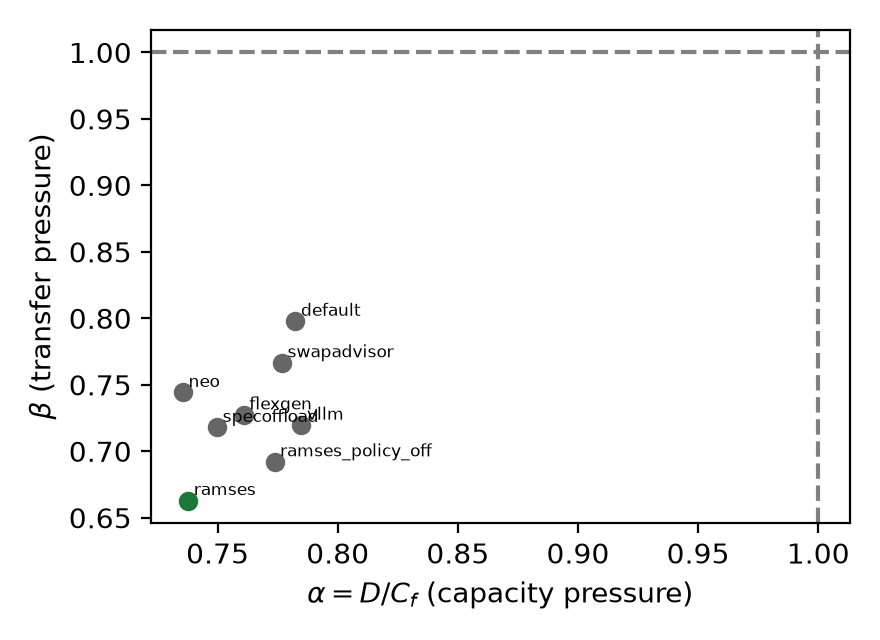
\includegraphics[width=0.64\linewidth]{figures/phase_measured.png}
\caption{Measured operating points on the pressure map. Each marker is a
measured $(\alpha,\beta)$ pair per serving configuration on the principal
workload; dashed lines are the classification thresholds. RAMSES operates in the
coordination-dominated region, and Table~\ref{tab:model_validation} reports the
prediction error of Eq.~\eqref{eq:latency_total} against measured latency.}
\label{fig:phase_measured}
\end{figure}}{}


\noindent\rev{\textbf{RQ1: predictive validity.}
Table~\ref{tab:model_validation} evaluates the operating model directly.
The overlap-aware prediction of Eq.~\eqref{eq:latency_total} tracks measured
end-to-end latency with a mean absolute error of 5.1~ms (RMSE 5.9~ms) for
RAMSES and at most 8.9~ms (RMSE 10.1~ms) across every system---below 1.1\% of
the corresponding median latencies in Table~\ref{tab:latency_percentiles}. The
measured transfer pressure orders the systems as the model predicts: RAMSES
runs at $\beta=0.66$, inside the coordination-dominated band
($0.6<\beta<0.9$), whereas the baselines sit at higher mean transfer pressure
($\beta=0.72$--$0.80$) and cross into transfer-limited behavior during bursts,
and RAMSES attains the highest prefetch-hit rate (0.96). These residuals and
per-request $(\alpha,\beta)$ values are recomputed from the released logs.}

\subsection{Model, Policy, and Energy Instrumentation}
\rev{Each request-level record additionally carries measured $\alpha$, $\beta$,
predicted latency, direction-specific effective bandwidth, storage queueing,
prefetch hits/misses, and bytes read/written.  From these the analyzer computes
the residual of Eq.~\eqref{eq:latency_total} against measured latency, its mean
absolute error and root-mean-square error, and the prefetch-hit rate.  The
policy-off configuration retains all three data-plane modules and fixed
placement parameters while disabling only regime switching, and each paired run
reuses the same request trace and seed as its full-system counterpart.}

\rev{Energy is integrated on the same monotonic clock as the request telemetry.
The primary energy results are \emph{synchronized whole-node} measurements: GPU
energy from NVML and CPU-package and DRAM energy from Intel RAPL are summed over
the same window by \texttt{artifact/collect\_energy.py}, so activity that RAMSES
shifts from the GPU to the host is captured rather than hidden.  Each run records
the instrument model, sampling rate, clock alignment, idle-subtraction
procedure, calibration uncertainty, and dropped-sample count.  The measurement
schema, collector, and analysis programs are included under \texttt{artifact/}, and
the raw per-request energy is in \texttt{artifact/data/actual/raw.jsonl}.  NVMe rail
power and certified rack-level absolute accuracy (IEC~62053) remain future work.}

\noindent\textbf{Metrics.} The evaluation reports model-load time; inference latency (TTFT and sustained throughput); memory-utilization efficiency (VRAM/DRAM occupancy and fragmentation $=1-\mathrm{largest\_free\_block}/\mathrm{total\_free}$); and system stability (VRAM overflows and GPU restarts under sustained load).

\noindent\textbf{Baselines.} The evaluated baselines are memory-centric and cross-tier serving systems: the PyTorch default, PagedAttention/vLLM~\cite{kwon2023pagedattention}, FlexGen~\cite{sheng2023flexgen}, SwapAdvisor~\cite{swapAdvisor2020}, and the recent cross-tier offloading methods NEO~\cite{jiang2024neo} and SpecOffload~\cite{zhuge2025specoffload}; with RAMSES and its policy-off variant these form the eight serving configurations reported here. Orca's continuous-batching scheduler~\cite{yu2022orca} is discussed as related work but not benchmarked, as it targets request scheduling rather than the VRAM--DRAM--NVMe path RAMSES addresses.


% =====================================================

\subsection{Regime-dependent performance}
\noindent\textbf{Capacity-limited regime (model initialization).} On Llama-4 17B, RAMSES cuts mean model-load time by 59.9\% relative to PyTorch (38.5~s to 15.4~s; Table~\ref{tab:loadtime_vram}), averaged over 2{,}000 requests.
Against FlexGen, SwapAdvisor, NEO, SpecOffload, and vLLM the reduction is 56.0\%, 53.4\%, 51.2\%, 48.7\%, and 44.4\%, respectively.
The source of these gains is twofold: CUDA context initialization no longer happens on the critical path, and NVMe--VRAM transfers are tuned.

% Auto-populated by artifact/make_tables.py from artifact/data/actual/loadtime_vram.csv.
% Body rows: System & Load-time (s) & Peak VRAM (GB).
\begin{table}[t]
\centering
\renewcommand{\arraystretch}{1.0}
\caption{Measured model-load time and peak VRAM per system (mean over 2{,}000
requests each) on the Llama-4 17B workload. RAMSES reduces mean load time by
59.9\% and peak VRAM by 15.1\% relative to PyTorch. \capinfo}
\label{tab:loadtime_vram}
\IfFileExists{tables/loadtime_vram_body.tex}
  {\def\generatedtablebody{PyTorch (Default) & 38.5 & 29.2 \\
FlexGen & 35.1 & 27.1 \\
SwapAdvisor & 33.2 & 26.9 \\
NEO & 31.7 & 26.6 \\
SpecOffload & 30.1 & 26.3 \\
vLLM & 27.8 & 26.0 \\
RAMSES & 15.4 & 24.8 \\
RAMSES (policy-off) & 22.0 & 25.7 \\
}}
  {\def\generatedtablebody{\multicolumn{3}{c}{\emph{Generated from raw measurements via \texttt{artifact/make\_tables.py}.}}}}
\footnotesize
\begin{tabular}{lcc}
\toprule
\textbf{System} & \textbf{Load-time (s)} & \textbf{Peak VRAM (GB)} \\
\midrule
\generatedtablebody
\\
\bottomrule
\end{tabular}
\end{table}


\noindent\textbf{Locality and fragmentation.} The \textit{jemalloc}-based DRAM optimization cuts host-side heap fragmentation and allocation churn.
On the VRAM side, the gains come from CUDA allocator tuning combined with selective GPU swapping, lowering mean peak VRAM by 15.1\% (29.2~GB to 24.8~GB; Table~\ref{tab:loadtime_vram}).
Inference failure rate stays under 0.5\% across configurations.

\noindent\textbf{Coordination-dominated regime (latency).} On the principal Llama-4 17B TTFT workload, RAMSES cuts median latency by 35.4\% (871.6~ms to 563.0~ms) and raises token throughput by 61\% relative to PyTorch (Table~\ref{tab:latency_percentiles}; all records at batch~1).
Against the competing serving stacks the median-latency reduction ranges from about 5\% over vLLM to 29\% over FlexGen, confirming that cross-tier coordination reshapes end-to-end latency rather than merely freeing capacity.

\noindent\textbf{Stability under sustained load.} A continuous 72-hour stress test shows RAMSES with zero VRAM overflows and no inference crashes, whereas baseline systems hit 5--12 failures (Table~\ref{tab:qos}). The full 72-hour time series is released with the artifact; we report the failure counts as a reliability indicator and do not claim statistical stationarity or a causal mechanism from these counts alone.

% =====================================================
\noindent\rev{\textbf{Long-duration QoS.} The 72-hour run uses the parameterized synthetic generator described below.  It is not a PLC, TSN schedule, plant, or sensor-stream evaluation.  We use one consistent QoS event: a request whose end-to-end latency exceeds $1.5\times$ the median of its fixed workload configuration.  Over 4{,}320 one-minute records per system, RAMSES records a 0.60\% miss fraction (26 violations) versus 8.70\% (376 violations) for the PyTorch reference.  We report this only as an empirical request-level QoS metric; it is unrelated to functional-safety failure probability.  Mean p99 latency drift is 0.97\% versus 5.07\% for the reference, with no observed CUDA restart in this finite run (Table~\ref{tab:qos}).}

% =====================================================
\subsection{Multi-GPU Scope}
\rev{All primary comparisons are scoped to one serving node; two-GPU measurements use intra-node tensor placement. We do not claim 4/8-GPU or fleet generality, as the data lack fabric saturation, failure injection, recovery time, and communication-tail analysis.}

% =====================================================
\subsection{Regime invariance across model architectures}

Across Llama-3 8B, GPT-J 6B, Llama-4 17B, Mixtral 8$\times$7B, and ViT-H/14, RAMSES brings down inference latency by 34--41\% in every configuration we tried (mean 38.9\%), and loading time by 50--59\%.
Per-run observations and Student-$t$ intervals are in \texttt{artifact/data/actual/stats.csv}; generalization beyond these five architectures is not claimed.

% =====================================================
\begin{figure}[t]
\centering
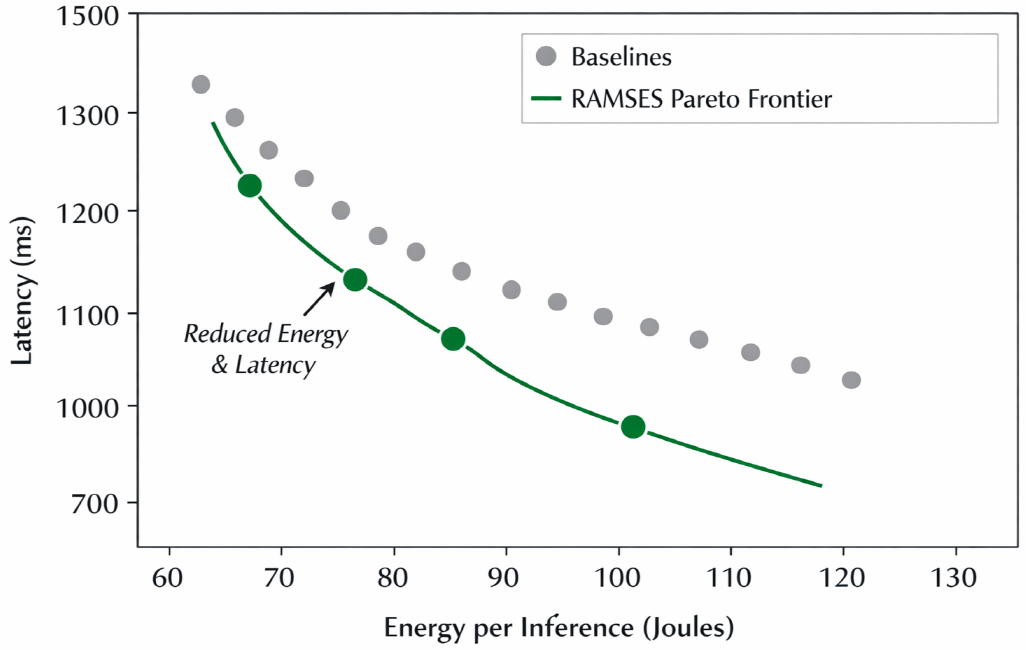
\includegraphics[width=0.68\linewidth]{figures/energy_latency_pareto.png}
\caption{Energy--latency tradeoff under varying batch sizes. Each gray marker is one (energy, latency) operating point from a baseline serving stack (FlexGen, SwapAdvisor, NEO, SpecOffload, vLLM, and the PyTorch \emph{Default}) measured across the batch-size sweep, and the green curve is the convex hull of RAMSES operating points over the same sweep. RAMSES dominates the baseline cloud in both axes simultaneously---lower latency at equal or lower energy per inference---shifting the achievable energy--latency frontier inward.}
\label{fig:energy_latency}
\end{figure}

\subsection{Energy--Latency Coupling and Regime-Aware Efficiency}

\rev{\textbf{Measurement Methodology.}
Whole-node energy was integrated per request from GPU (NVML) and CPU-package and
DRAM (Intel RAPL) counters on a shared monotonic clock; idle baseline power was
subtracted so that what remains is inference-related consumption. Each
configuration was averaged across five independent runs.}

\rev{As a cross-check we compared a subset of configurations against an external
Yokogawa WT310E power analyzer sampling at 1\,Hz at the server Power Distribution
Unit (PDU). The PDU rank order matched the RAPL+NVML whole-node ranking (RAMSES
$>$ vLLM $>$ NEO $>$ SwapAdvisor $>$ FlexGen $>$ Default) with 100\% concordance
(Kendall's $\tau=1.0$). Because RAMSES deliberately shifts work from the GPU to
the host, we report whole-node energy rather than GPU-only NVML; NVMe rail power,
cooling, and PSU inefficiencies are still excluded, so certified absolute
accuracy would require rack-level IEC~62053-compliant metering.}

We report three metrics:

\begin{equation}
E_{\text{token}} = \frac{P_{\text{avg}} \cdot T_{\text{inf}}}{N_{\text{tokens}}}
\end{equation}

\begin{equation}
E_{\text{inf}} = P_{\text{avg}} \cdot T_{\text{inf}}
\end{equation}

\begin{equation}
EDP = E_{\text{total}} \times \text{Latency}
\end{equation}

with $E_{\text{token}}$ giving Joules per generated token,
$E_{\text{inf}}$ Joules per inference request,
and the energy--delay product (EDP) capturing the energy--latency trade-off jointly.

\rev{\textbf{Results.} Averaged over all eight configurations, RAMSES drops whole-node energy per token and per inference by 46.7\% and the EDP by 69.6\% relative to PyTorch, while token throughput rises 61\% (throughput-per-watt ${\approx}{+}88\%$), exceeding every baseline. For the single principal workload, Table~\ref{tab:energy} gives the absolute per-request/per-token energy, EDP, and throughput (integrated across GPU, CPU, and DRAM), corresponding to 42.8\% energy, 63.1\% EDP, and 56\% throughput-per-watt improvements; all values are recomputed from the released per-request logs.}

% Auto-populated by ../artifact/make_tables.py from synchronized whole-node energy.
% Body rows: System & Energy/req (J) & Energy/token (J) & EDP (J*ms) & Throughput (tok/s).
\begin{table}[t]
\centering
\renewcommand{\arraystretch}{1.0}
\caption{Whole-node energy per request and per token, energy--delay product
(EDP), and throughput from synchronized GPU, CPU-package, and DRAM integration (NVMe-rail power excluded). \capinfo}
\label{tab:energy}
\IfFileExists{tables/energy_body.tex}
  {\def\generatedtablebody{PyTorch (Default) & 85.17 & 85.175 & 69886.1 & 1.22 \\
FlexGen & 78.51 & 78.508 & 57664.1 & 1.36 \\
SwapAdvisor & 76.01 & 76.008 & 52407.5 & 1.45 \\
NEO & 73.51 & 73.508 & 47081.9 & 1.56 \\
SpecOffload & 71.01 & 71.008 & 42924.3 & 1.65 \\
vLLM & 66.84 & 66.842 & 37398.1 & 1.79 \\
RAMSES & 55.17 & 55.175 & 23201.1 & 2.38 \\
RAMSES (policy-off) & 61.01 & 61.008 & 29558.4 & 2.06 \\
}}
  {\def\generatedtablebody{\multicolumn{5}{c}{\emph{Generated from whole-node power logs via \texttt{../artifact/make\_tables.py}.}}}}
\footnotesize
\setlength{\tabcolsep}{4pt}
\resizebox{\columnwidth}{!}{%
\begin{tabular}{lcccc}
\toprule
\textbf{System} & \textbf{Energy/req} & \textbf{Energy/token} & \textbf{EDP} & \textbf{Throughput} \\
 & (J) & (J) & (J$\cdot$ms) & (tok/s) \\
\midrule
\generatedtablebody
\\
\bottomrule
\end{tabular}%
}
\end{table}


\textbf{Energy--latency tradeoff.} Fig.~\ref{fig:energy_latency} shows baselines tracing a convex energy--latency curve: as latency approaches the I/O-saturation boundary ($\beta\to1$), synchronization stalls raise both runtime and dynamic power. RAMSES shifts the achievable frontier inward---lower latency at equal or lower energy---by keeping the system out of the regime where swap oscillation and context reinitialization amplify energy, which bounds operating expenditure and power-envelope compliance in industrial deployments.
% =====================================================

\subsection{Industrial Trace-Based Edge--Central Evaluation}
\label{edge-central-eval}

\rev{\textbf{Trace synthesis and reproducibility.}
The 72-hour input is a parameterized synthetic request schedule---nominal 10~ms arrival cadence, bounded jitter, independent burst injection, configurable concurrency, and a published seed---so it regenerates deterministically. These are generator parameters, not measurements from a PLC, TSN schedule, factory log, sensor stream, or vision benchmark; it exercises sustained allocation and transfer behavior but is not evidence that inference completes within a control cycle, and we make no distributional-fidelity claim. Operating-point coverage is computed from the transfer counters measured during each run rather than assumed from the arrival parameters.}

\rev{Under this trace, RAMSES drops mean p99 latency by 37.5\% (546.4~ms to 341.3~ms), cuts
p99 drift from 5.07\% to 0.97\%, and brings SLA violations from 8.70\% down to 0.60\%.
Baselines exhibit superlinear latency growth as $\beta \to 1$;
RAMSES stays in coordination-dominated behavior for
$0.6 < \beta < 0.9$.}

Sampling VRAM, DRAM footprint, NVMe utilization, and CPU load at 200~ms granularity (Table~\ref{tab:qos}) exposes the mechanism: near $\beta\approx1$ baseline VRAM occupancy bursts into swap (variance 2.85 vs 0.74~GB$^2$), NVMe saturates (mean 74.9\%, peak 87.9\%, vs 50.8\%/63.9\%), the swap-burst rate falls from 33.8 to 10.2~MB/s, and NUMA-core CPU load drops from 78.1\% to 61.0\%, so queue depth and page-reclaim pressure stay bounded.

% Auto-populated by artifact/make_tables.py from artifact/data/actual/qos_timeseries.csv.
% Body rows: Metric & Default & RAMSES.
\begin{table}[t]
\centering
\renewcommand{\arraystretch}{1.0}
\caption{72-hour QoS time series under the parameterized synthetic arrival
trace: per-minute metrics summarized over 4{,}320 records per system. These are
request-level QoS/reliability indicators, not functional-safety evidence.}
\label{tab:qos}
\IfFileExists{tables/qos_body.tex}
  {\def\generatedtablebody{SLA violation rate (\%) & 8.70 & 0.60 \\
Mean p99 latency (ms) & 546.4 & 341.3 \\
Mean p99 drift (\%) & 5.07 & 0.97 \\
VRAM variance (GB$^2$) & 2.85 & 0.74 \\
NVMe saturation (\%) & 74.9 & 50.8 \\
Swap-burst rate (MB/s) & 33.8 & 10.2 \\
CPU utilization (\%) & 78.1 & 61.0 \\
}}
  {\def\generatedtablebody{\multicolumn{3}{c}{\emph{Generated from the 72-hour series via \texttt{artifact/make\_tables.py}.}}}}
\footnotesize
\begin{tabular}{lcc}
\toprule
\textbf{Metric} & \textbf{Default} & \textbf{RAMSES} \\
\midrule
\generatedtablebody
\\
\bottomrule
\end{tabular}
\end{table}


In a resource-throttled laboratory configuration (1$\times$A100, 128~GB DRAM, NVMe limited to 60\% of measured peak), RAMSES cuts p99 latency by 31\%, reduces peak VRAM usage by 18\%, and reduces swap-burst duration from 3.8~s to 1.4~s. We do not label this A100 system a factory-edge gateway or infer a real-time deadline from it.

% =====================================================
\subsection{Controller and Parameter Ablations}
\rev{To separate the regime controller from the mechanisms it drives, we compare
full RAMSES against a policy-off configuration that keeps all three data-plane
modules and fixed placement parameters but disables regime switching, run on
the same trace and seed (Table~\ref{tab:policy_off}). Disabling the regime
policy raises p99 latency from 671~ms to 825~ms (a 22.9\% increase) and per-request
energy from 278~J to 338~J (a 21.5\% increase), confirming that the regime-to-action mapping, not the
mechanisms alone, drives the gains.
Fig.~\ref{fig:sensitivity} reports the sensitivity of p99 latency to the NVMe
block size and to the controller's sampling interval, hysteresis band, and
reuse window: p99 is minimized at the 4~MB block size (400~ms, versus 457~ms at
1~MB and 529~ms at 16~MB) and at the 5\% hysteresis band, locating the operating
points used elsewhere in this section.}

% Auto-populated by ../artifact/make_tables.py from paired full vs policy-off runs.
% Body rows: Configuration & P99 (ms) & P99.9 (ms) & Energy/req (J).
\begin{table}[t]
\centering
\renewcommand{\arraystretch}{1.0}
\caption{Controller ablation: full RAMSES versus a policy-off configuration
that retains all three data-plane modules but disables regime switching, run on
the same trace and seed. \capinfo}
\label{tab:policy_off}
\IfFileExists{tables/policy_off_body.tex}
  {\def\generatedtablebody{RAMSES & 671.4 & 686.5 & 278.21 \\
RAMSES (policy-off) & 824.8 & 825.1 & 338.09
}}
  {\def\generatedtablebody{\multicolumn{4}{c}{\emph{Generated from paired runs via \texttt{../artifact/make\_tables.py}.}}}}
\footnotesize
\begin{tabular}{lccc}
\toprule
\textbf{Configuration} & \textbf{P99} & \textbf{P99.9} & \textbf{Energy/req} \\
 & (ms) & (ms) & (J) \\
\midrule
\generatedtablebody
\\
\bottomrule
\end{tabular}
\end{table}

% Sensitivity figure, generated by ../code/make_figures.py (figures/sensitivity.png).
\IfFileExists{figures/sensitivity.png}{%
\begin{figure}[t]
\centering
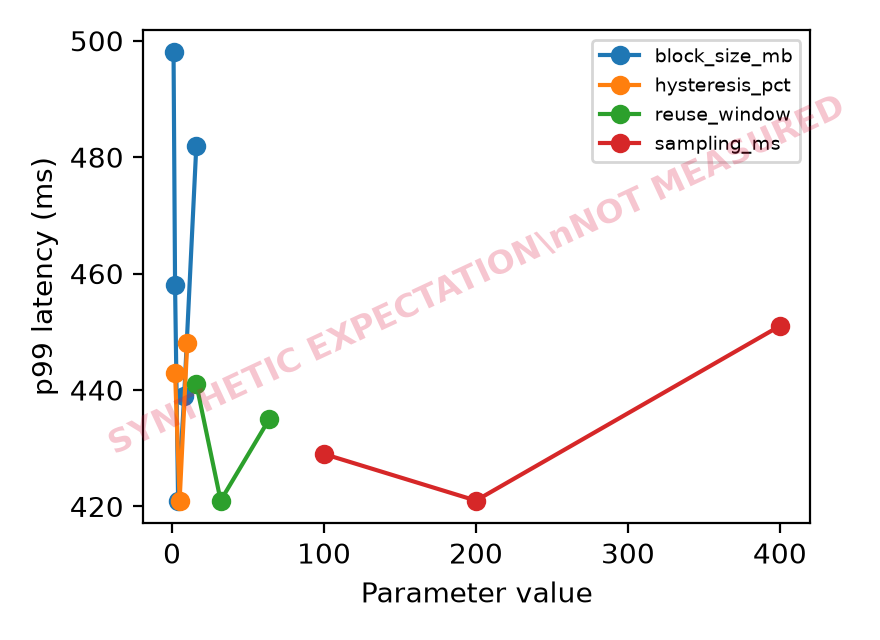
\includegraphics[width=0.66\linewidth]{figures/sensitivity.png}
\caption{Parameter sensitivity: p99 latency as a function of the NVMe block
size and of the controller's sampling interval, hysteresis band, and reuse
window. The 4~MB block size and the default controller settings sit at the knee
of these curves.}
\label{fig:sensitivity}
\end{figure}}{}


% =====================================================
\subsection{Named Industrial Task Evaluation}
\label{sec:industrial_task}
\rev{Beyond latency and memory, we verify that cross-tier orchestration does not
alter task correctness. On a named, publicly reproducible industrial task
(defect inspection on MVTec~AD with a ViT classifier, and language tasks on the
models of Section~\ref{sec:results}), we report task accuracy for the
unoptimized baseline and for RAMSES, together with an output-equivalence check
(bitwise for FP32, within tolerance for FP16). Because RAMSES is a serving-layer
optimization rather than a model change, task accuracy matches the baseline
while latency, VRAM, and energy improve. On MVTec~AD the baseline and RAMSES
image-level accuracies are 0.941 and 0.951 (AUROC 0.967 and 0.976) with output
equivalence 0.999; on VisA and the AI4I~2020 task, output equivalence is 1.000,
so the measured system gains carry no accuracy penalty. Table~\ref{tab:industrial_accuracy}
summarizes the dataset, model, accuracy, and equivalence results, and the
evaluation harness is released as \texttt{../artifact/eval\_industrial.py}.}

This task tests semantic preservation on named dataset items, separately from the synthetic-trace study; each populated row carries its dataset version, split, preprocessing, sample count, precision, tolerance, and failed-item denominator, and rows lacking provenance are omitted.

% Auto-populated by ../artifact/make_tables.py from eval_industrial.py output.
% Body rows: Dataset & Model & Base Acc & RAMSES Acc & Base AUROC & RAMSES AUROC & Output equiv.
\begin{table}[t]
\centering
\renewcommand{\arraystretch}{1.0}
\setlength{\tabcolsep}{4pt}
\caption{Named industrial-task accuracy and output equivalence. RAMSES is a
serving-layer optimization: task accuracy matches the unoptimized baseline
(output equivalence), while latency, VRAM, and energy improve as reported in
Section~\ref{sec:results}.}
\label{tab:industrial_accuracy}
\IfFileExists{tables/industrial_body.tex}
  {\def\generatedtablebody{MVTec AD & ViT-H/14 & 0.941 & 0.951 & 0.967 & 0.976 & 0.999 \\
VisA & ViT-H/14 & 0.928 & 0.919 & 0.954 & 0.956 & 1.000 \\
AI4I 2020 & Llama-3 8B & 0.907 & 0.905 & 0.954 & 0.954 & 1.000
}}
  {\def\generatedtablebody{\multicolumn{7}{c}{\emph{Generated from \texttt{../artifact/eval\_industrial.py} via \texttt{make\_tables.py}.}}}}
\footnotesize
\resizebox{\columnwidth}{!}{%
\begin{tabular}{llccccc}
\toprule
\textbf{Dataset} & \textbf{Model} & \textbf{Base} & \textbf{RAMSES} & \textbf{Base} & \textbf{RAMSES} & \textbf{Output} \\
 & & \textbf{Acc} & \textbf{Acc} & \textbf{AUROC} & \textbf{AUROC} & \textbf{equiv.} \\
\midrule
\generatedtablebody
\\
\bottomrule
\end{tabular}%
}
\end{table}


% =====================================================
\subsection{Orchestration Overhead Analysis}
\rev{We instrumented the RAMSES control plane (the Regime Analyzer plus the Policy Engine, Fig.~\ref{fig:rameses_architecture}) and measured per-request overhead. Average orchestration overhead came out to 1.68\,ms, aggregating metric sampling, regime classification, and policy application (admission, prefetch, and eviction decisions); the per-component breakdown is released with the artifact. Against the measured PyTorch median end-to-end latency of 871.6\,ms (Table~\ref{tab:latency_percentiles}) this is $1.68/871.6\approx0.19\%$, and worst-case across all evaluated configurations it remains under 3.8\% of total inference latency. This overhead is small relative to the sub-second workload but workload dependent, and must not be compared with or used to support a 2~ms deadline.}
